\section{Módulo localización de zonas turísticas}

\subsection{Objetivo}
El objetivo de este módulo es poder mostrar las zonas turísticas que se tienen registradas dentro del sistema, en un dispositivo móvil.

\subsection{Diseño}

Para este módulo se diseñó una vista en la que se pudieran ver listadas las zonas turisticas que se encuentran dentro del sistema

\subsection{Desarrollo}

Para el desarrollo de la API se utilizó el formato JSON para el envío de datos.


\subsection{Resultados}

La Figura \ref{fig:zonasT} muestra el resultado que se obtuvo por la implemetación del módulo de registro, en ella se puede ver como se integró el botón \textit{Sign in with Apple} provisto por Apple. \\

\begin{figure}[htbp]
	\begin{center}
		\fbox{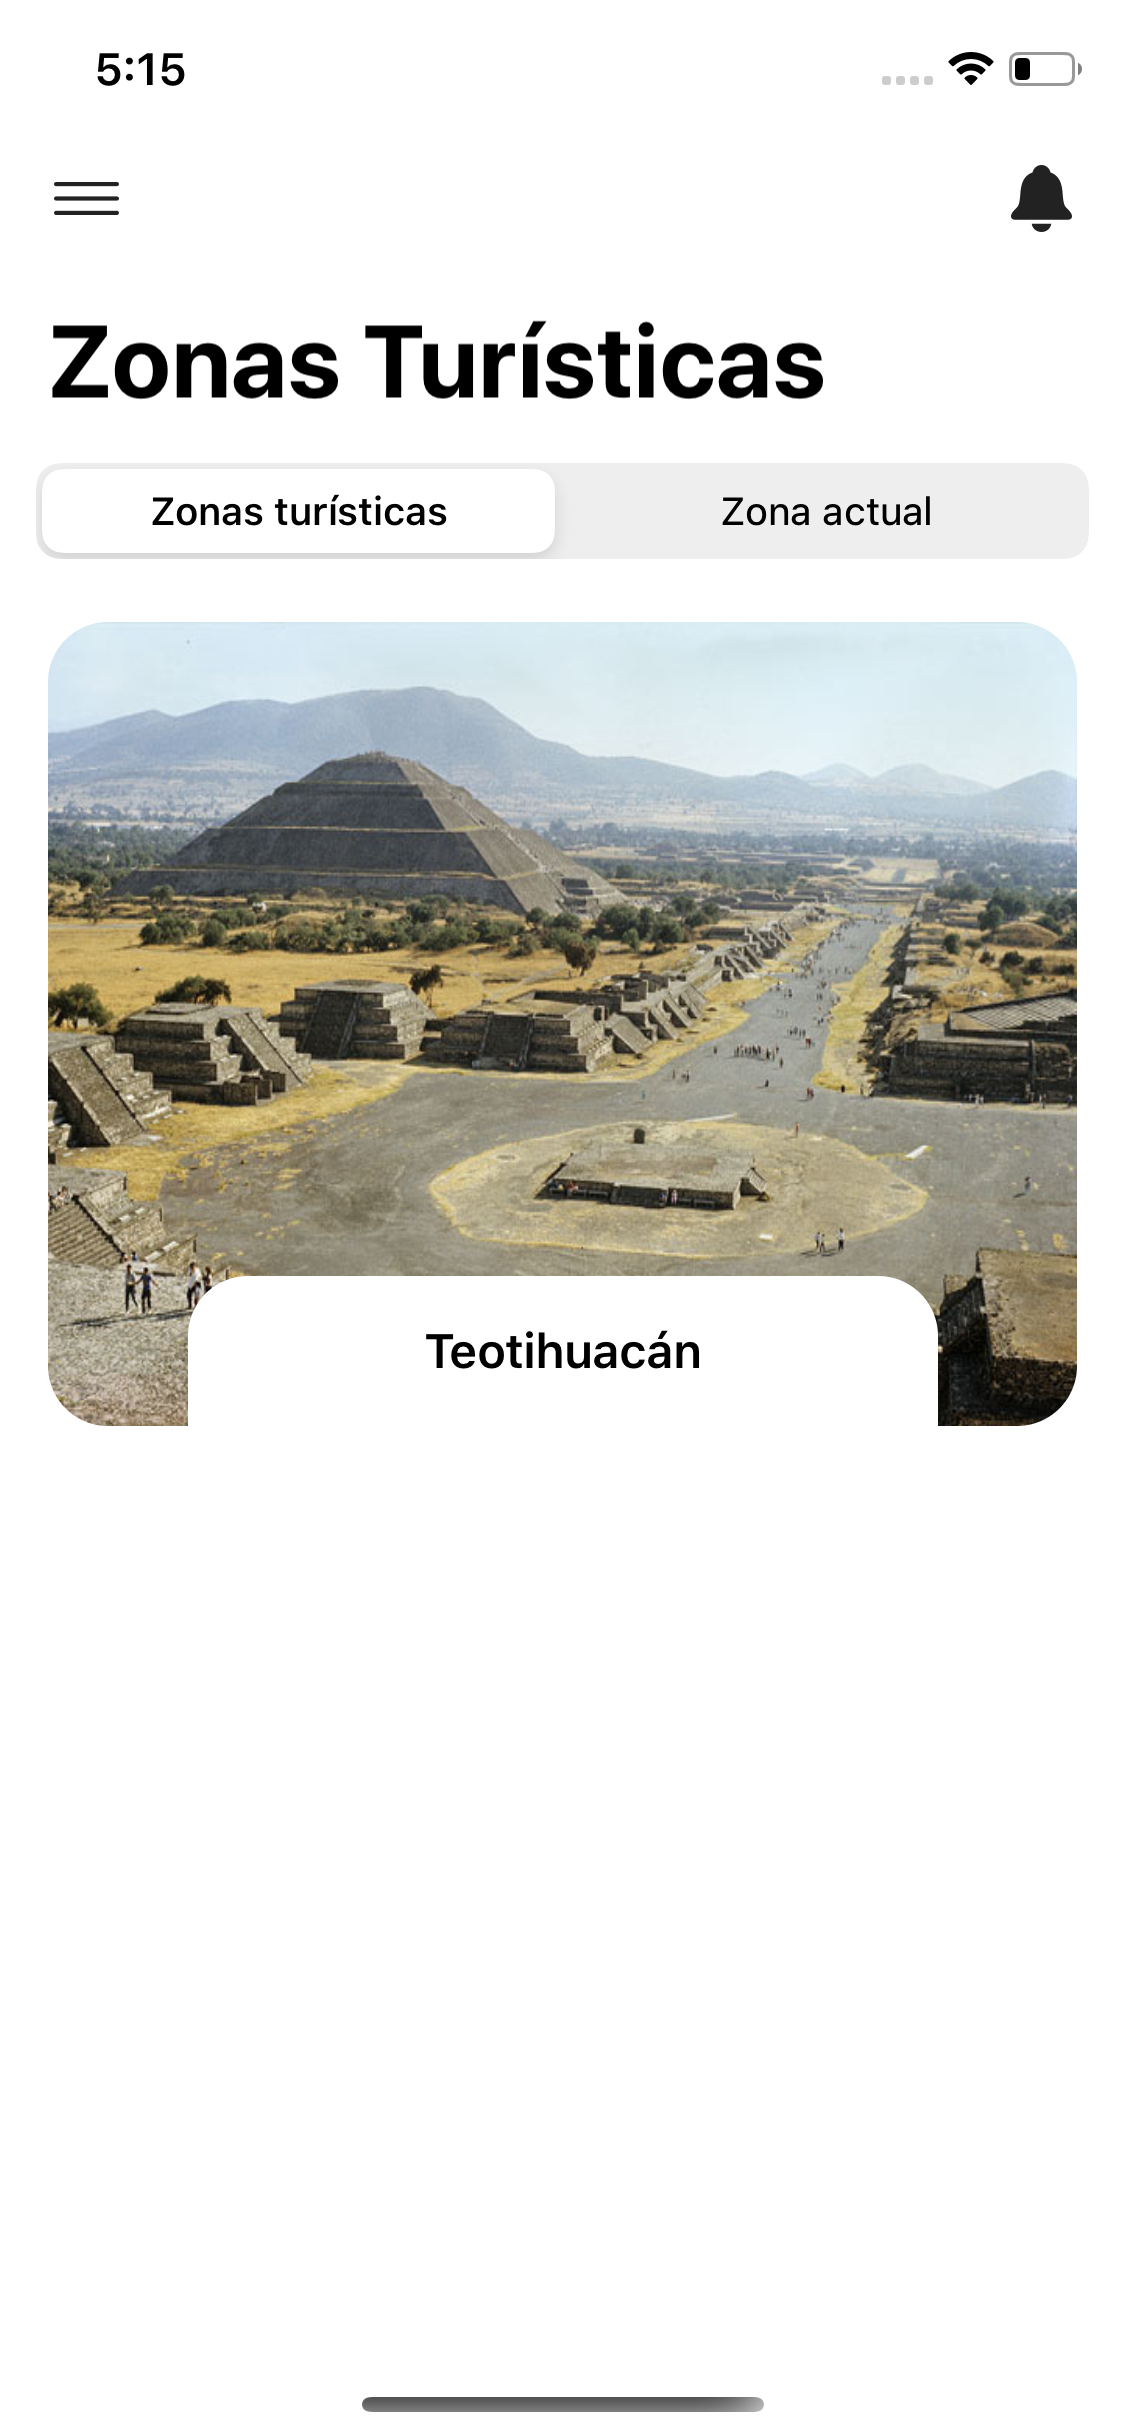
\includegraphics[scale = .1]{implementacion/localizacion/images/zonas}}
		\caption{Resultado módulo lozalización de zonas turísticas}
		\label{fig:zonasT}
	\end{center}
\end{figure}